\documentclass[11pt,fleqn]{article}
\usepackage{../cs188,latexsym,epsf, amsmath,amsfonts,graphicx,url,multicol}
\lecture{2}
\def\title{Note \the\lecturenumber}
\begin{document}
\maketitle


\iffalse
\documentclass[11pt,fleqn]{article}
\usepackage{latexsym,epsf,amsmath,amsfonts,graphicx,url}

\title{Note 2}

\newcommand{\F}{\mathbb{F}}
\newcommand{\Z}{\mathbb{Z}}
\newcommand{\Q}{\mathbb{Q}}
\newcommand{\R}{\mathbb{R}}
\newcommand{\C}{\mathbb{C}}

\begin{document}

\maketitle
\fi

\section*{Constraint Satisfaction Problems}
In the previous section, we learned how to find optimal solutions to search problems, a type of \textbf{planning problem}. Now, we'll learn about solving a related class of problems, \textbf{constraint satisfaction problems} (CSPs). Unlike search problems, CSPs are a type of \textbf{identification problem}, problems in which we must simply identify whether a state is a goal state or not, with no regard to how we arrive at that goal. CSPs are defined by three factors:
	\begin{enumerate}
		\item \textit{Variables} - CSPs possess a set of $N$ variables $X_1, ..., X_N$ that can each take on a single value from some defined set of values.
		\item \textit{Domain} - A set representing all possible values that a CSP variable can take on.
		\item \textit{Constraints} - Constraints define restrictions on the values of variables, potentially with regard to other variables.
	\end{enumerate}
Consider the $N$-queens identification problem: given an $N \times N$ chessboard, can we find a configuration in which to place $N$ queens on the board such that no two queens attack each another?
\begin{center}
	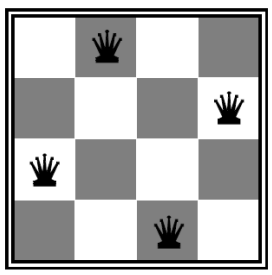
\includegraphics[width=3.7cm]{img/n-queens}
\end{center}
We can formulate this problem as a CSP as follows:
	\begin{enumerate}
		\item \textit{Variables} - $X_{ij}$, with $0 \leq i, j < N$. Each $X_{ij}$ represents a grid position on our $N \times N$ chessboard, with $i$ and $j$ specifying the row and column number respectively.
		\item \textit{Domain} - $\{0, 1\}$. Each $X_{ij}$ can take on either the value $0$ or $1$, a boolean value representing the existence of a queen at position $(i, j)$ on the board.
		\item \textit{Constraints} - 
			\begin{itemize}
				\item $\forall i,j,k \:\: (X_{ij}, X_{ik}) \in \{(0, 0), (0, 1), (1, 0)\}$. This constraint states that if two variables have the same value for $i$, only one of them can take on a value of 1. This effectively encapsulates the condition that no two queens can be in the same row.
				\item $\forall i,j,k \:\: (X_{ij}, X_{kj}) \in \{(0, 0), (0, 1), (1, 0)\}$. Almost identically to the previous constraint, this constraint states that if two variables have the same value for $j$, only one of them can take on a value of 1, encapsulating the condition that no two queens can be in the same column.
				\item $\forall i,j,k \:\: (X_{ij}, X_{i+k,j+k}) \in \{(0, 0), (0, 1), (1, 0)\}$. With similar reasoning as above, we can see that this constraint and the next represent the conditions that no two queens can be in the same major or minor diagonals, respectively.
				\item $\forall i,j,k \:\: (X_{ij}, X_{i+k,j-k}) \in \{(0, 0), (0, 1), (1, 0)\}$.
				\item $\sum\limits_{i,j}X_{ij} = N$. This constraint states that we must have exactly $N$ grid positions marked with a $1$, and all others marked with a $0$, capturing the requirement that there are exactly $N$ queens on the board.
			\end{itemize}
	\end{enumerate}
Constraint satisfaction problems are \textbf{NP-complete}, which loosely means that there exists no known algorithm for finding solutions to them in polynomial time. Given a problem with $N$ variables with domain of size $O(d)$ for each variable, there are $O(d^N)$ possible assignments, exponential in the number of variables. We can often get around this caveat by formulating CSPs as search problems, defining states as \textbf{partial assignments} (variable assignments to CSPs where some variables have been assigned values while others have not). Correspondingly, the successor function for a CSP state outputs all states with one new variable assigned, and the goal test verifies all variables are assigned and all constraints are satisfied in a given state. Constraint satisfaction problems tend to have significantly more structure than traditional search problems, and we can exploit this structure by combining the above formulation with appropriate heuristics to hone in on solutions in a feasible amount of time.

\subsection*{Constraint Graphs}
Let's introduce a second CSP example: map coloring. Map coloring solves the problem where we're given a set of colors and must color a map such that no two adjacent states or regions have the same color.
	\begin{center}
		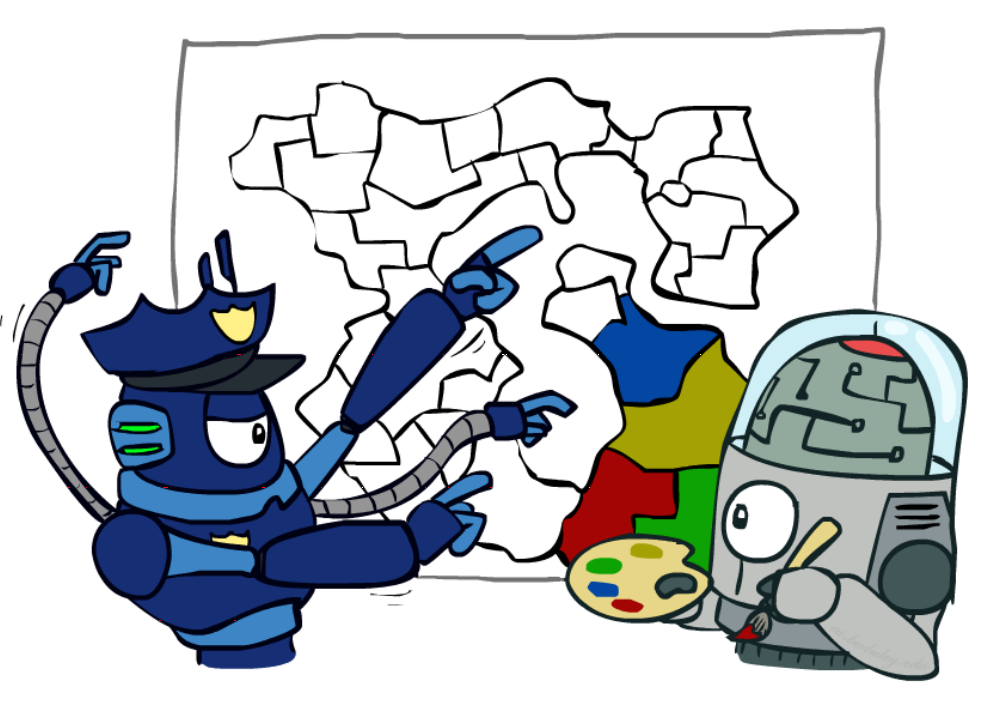
\includegraphics[width=7.5cm]{img/map-coloring-comic}
	\end{center}
Constraint satisfaction problems are often represented as constraint graphs, where nodes represent variables and edges represent constraints between them. There are many different types of constraints, and each is handled slightly differently:
\begin{itemize}
	\item \textit{Unary Constraints} - Unary constraints involve a single variable in the CSP. They are not represented in constraint graphs, instead simply being used to prune the domain of the variable they constrain when necessary.
	\item \textit{Binary Constraints} - Binary constraints involve two variables. They're represented in constraint graphs as traditional graph edges.
	\item \textit{Higher-order Constraints} - Constraints involving three or more variables can also be represented with edges in a CSP graph, they just look slightly unconventional.
\end{itemize} 
Consider map coloring the map of Australia:
	\begin{center}
		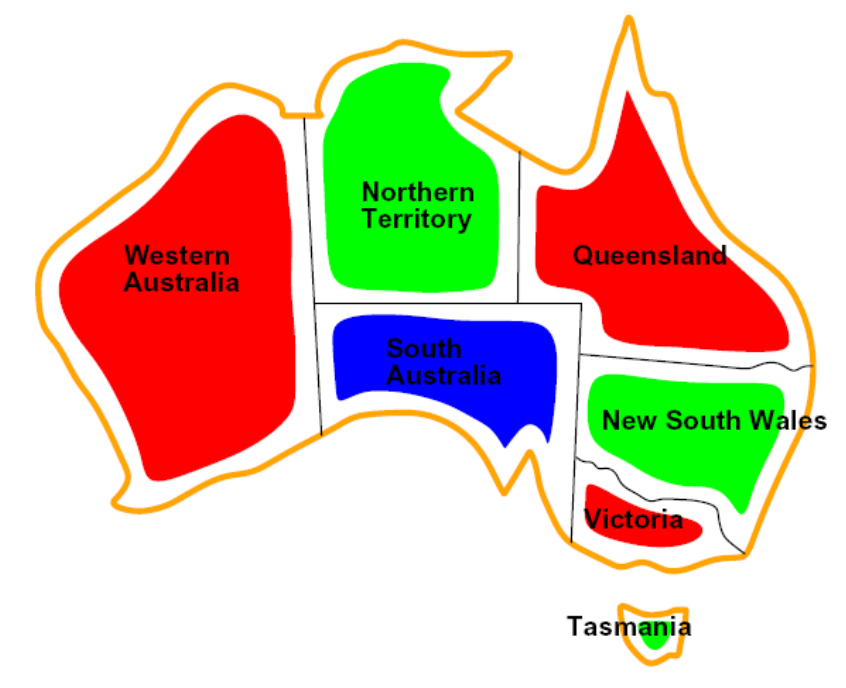
\includegraphics[width=7.5cm]{img/australia-map}
	\end{center}
As we can see, Western Australia is adjacent to Northern Territory and South Australia. Similarly generating adjacency pairs for every territory, we can generate the constraint graph for the map coloring of Australia as follows:
	\begin{center}
		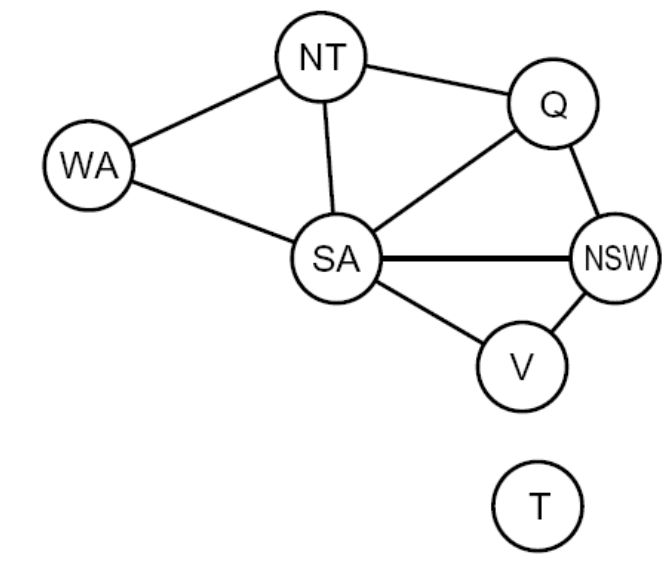
\includegraphics[width=7.5cm]{img/australia-graph}
	\end{center}
The value of constraint graphs is that we can use them to extract valuable information about the structure of the CSPs we are solving. By analyzing the graph of a CSP, we can determine things about it like if it's sparsely or densely connected/constrained and whether or not it's tree-structured. We'll cover this more in depth as we discuss solving constraint satisfaction problems in more detail.

\section*{Solving Constraint Satisfaction Problems}
Constraint satisfaction problems are traditionally solved using a search algorithm known as \textbf{backtracking search}. Backtracking search is an optimization on depth first search used for constraint satisfaction, with improvements coming from two main principles:
	\begin{enumerate}
		\item Fix an ordering for variables, and select values for variables in this order. Because assignments are commutative (e.g. assigning $WA = Red,\:\: NT = Green$ is identical to $NT = Green,\:\: WA = Red$), this is valid.
		\item When selecting values for a variable, only select values that don't conflict with any previously assigned values. 
	\end{enumerate}

The psuedocode for how recursive backtracking works is presented below:
	\begin{center}
		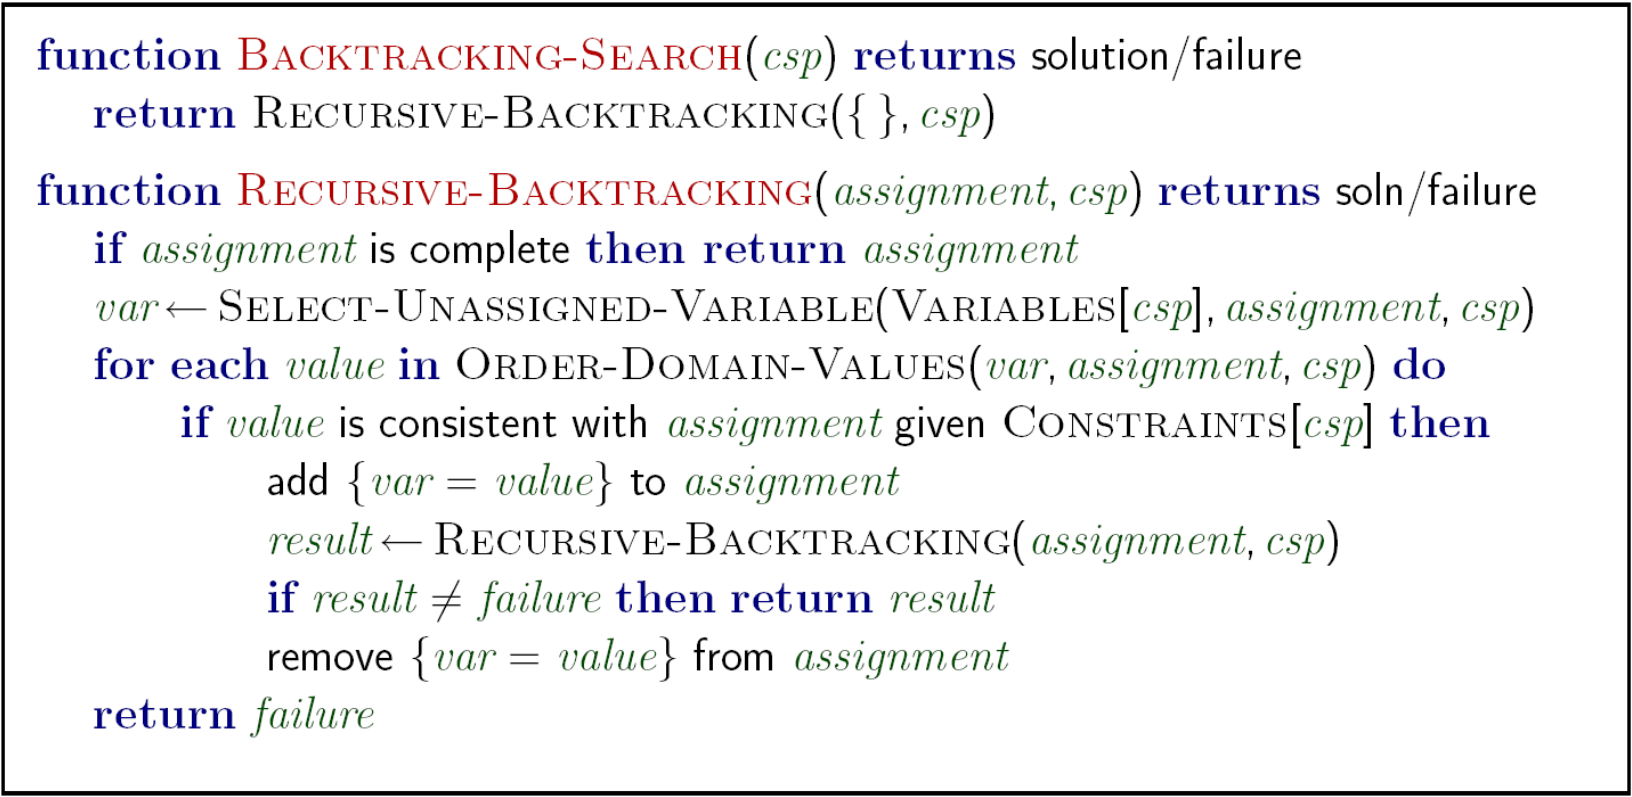
\includegraphics[width=12cm]{img/backtracking-search-pseudo.png}
	\end{center}
For a visualization of how it works, consider the partial search trees for both depth first search and backtracking search in map coloring:
	\begin{center}
		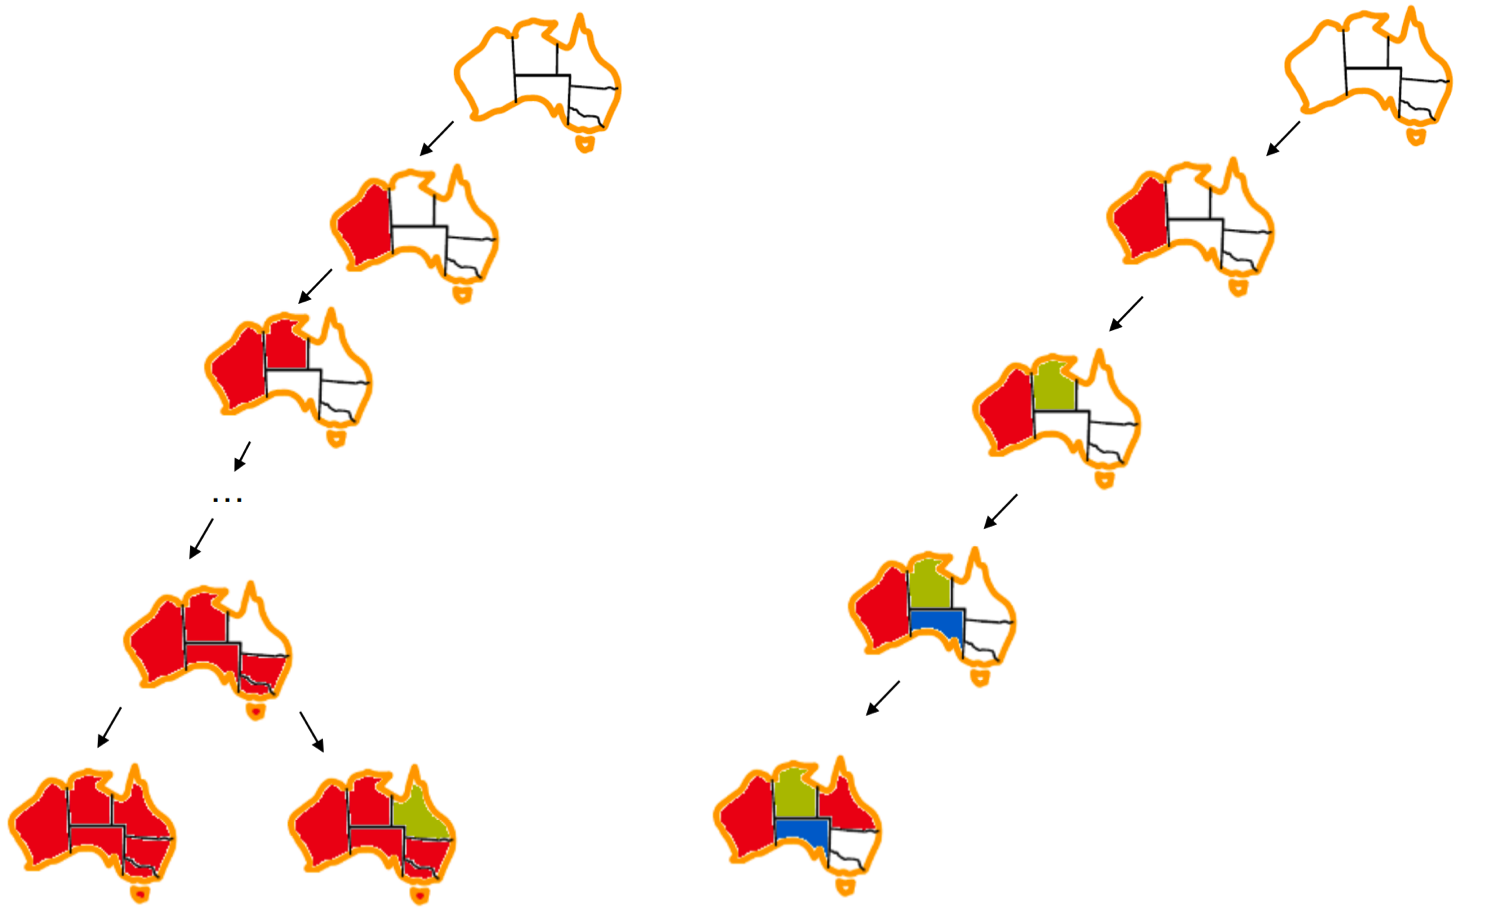
\includegraphics[width=12cm]{img/dfs-vs-backtracking.png}
	\end{center}
Note how DFS regretfully colors everything red before ever realizing the need for change, and even then doesn't move too far in the right direction towards a solution. On the other hand, backtracking search prunes the domains of unassigned variables immediately, leading to a significantly less backtracking. Though backtracking search is a vast improvement over the brute-forcing of depth first search, we can get more gains in speed still with further improvements through filtering, variable/value ordering, and structure explotation. 

\subsection*{Filtering}
		-filtering: keep track of domains for unassigned variables and eliminate bad options
		-forward checking
		-constraint propogation - detect failures early by reasoning between constraints (arc consistency)
			-for this provide example, and then explain keyness
			-can be run as a pre/postprocessor any assignment
			-arc consistency is much more expensive than forward checking, but is more key, so you need to weigh these pros and cons in problem
			-arc consistency pseudocode
				runtime: $O(n^2 d^3), can be reduced to O(n^2 d^2)$
			-solving a CSP is still np hard because even after enforcing arc consistency, can have one, more than one, or zero solutions and not know which one (EXAMPLE)
			-k consistency - increasing degrees of consistency
				1 consistency = node consistency
				2 consistency = arc consistency
				k consistency = for any group of k nodes, any assignment to k-1 group implies a possible assignment to the kth node
				strong k consistency - implies k, k-1, k-1, ..., 1 consistency
			implication of this is that strong-n consistency means we can solve without backtracking! easy to show, explain why this is
	

\subsection*{Ordering}
	We've delineated that when solving a CSP, we fix some ordering for both the variables and values involved. In practice, it's often much more effective to compute the next variable and corresponding value "on the fly" with two broad ideas, \textbf{minimum remaining values} and \textbf{least constraining value}:
		\begin{itemize}
			\item \textit{Minimum Remaining Values (MRV)} - When selecting which variable to assign next, using an MRV policy chooses whichever unassigned variable has the fewest valid remaining values (the \textit{most constrained variable}). This is intuitive in the sense that the most constrained variable is most likely to run out of possible values and trigger a backtrack, and so it's best to assign a value to it earlier than later.
			\item \textit{Least Constraining Value (LCV)} - Similarly, when selecting which value to assign next, a good policy to implement is to select the value that rules out the fewest values in the remaining unassigned values. Notably, this requires additional computation (e.g. rerunning arc consistency or other filtering methods for each value to find the LCV), but can still yield speed gains depending on the use case.
		\end{itemize}

\subsection*{Structure}
	-structure: is there a way we can exploit the problem based on the structure of the csp (constraint graph)
		-extreme case: independent subproblems are identifiable as connected components of constraint graph
			-lets say we can break up graph into components with c variables each, then runtime is $$O((n/c) d^c) because d^c assignments per connected component and n/c$$ connected components
			-something thats linear in n and only exponential in c, which is typically much smaller than n
			-provide example of gainz, which is present in slides

		-tree structured csp
			-if a csp has no loops, it can be solved in time $$O(nd^2)$$
			-genral csps have worst case runtimes of $$O(d^n)$$, so HUGE improvement
			-algorithm for tree structured CSPs
				-backwards pass, forwards pass
			 	-backwards enforce arc consistency backwards after linearizing
			 	-forwards pass, just assign (think about WHY this works and explain)
		-cutset conditioning: find the smallest number of things to remove such that everything is a tree thats remaining and use tree algorithm

\subsection*{Iterative Improvement}
	-iterative improvement
		-its often effective in practice idk just touch on this lightly


\section*{Summary}
	mention how CSPs are still NP complete problems and are hard and all of these things are really not efficient algorithms in and of themselves but rather are really just heuristics that can make arriving at a solution faster

	talk somewhere in general CSP solving section that we fix some ordering for variables and some ordering for values to try


\end{document}